% Provenance (never printed): enseignement scientifique premiere (2019),
% "La Terre, un astre singulier" (the place of the Earth) and the old seconde
% SVT "La planete Terre, une planete habitable" (conditions for liquid water,
% the habitable zone); see sources/book2/PROVENANCE.md. Every temperature,
% phase boundary and habitable-zone limit is computed in
% figdata/grade-10/planet_temperatures.py.
\chapter{宜居行星}\label{ch:g10:habitable-planet}

三颗岩质行星并排绕太阳运行。金星表面的
大气如此稠密，压强是地球上的九十二倍，
温度高得惊人——超过 \qty{460}{\degreeCelsius}——足以使铅熔化。
火星上稀薄的大气，压强不足我们这里的百分之一，而且
平均温度远低于冰点。二者之间，地球拥有
海洋、降雨与生命。这三颗行星形成于环绕年轻太阳的同一气体与
尘埃圆盘，由大致相同的岩石构成。为何命运如此不同？
本章探讨：什么决定行星的温度，什么使行星能保有大气，
水在何种条件下能呈液态，以及在何处能找到这些条件，
包括太阳周围和其他恒星周围。
% ledger: nasa:venus-atm, nasa:mars-atm, planet:Venus.Tmean

\begin{omfigure}
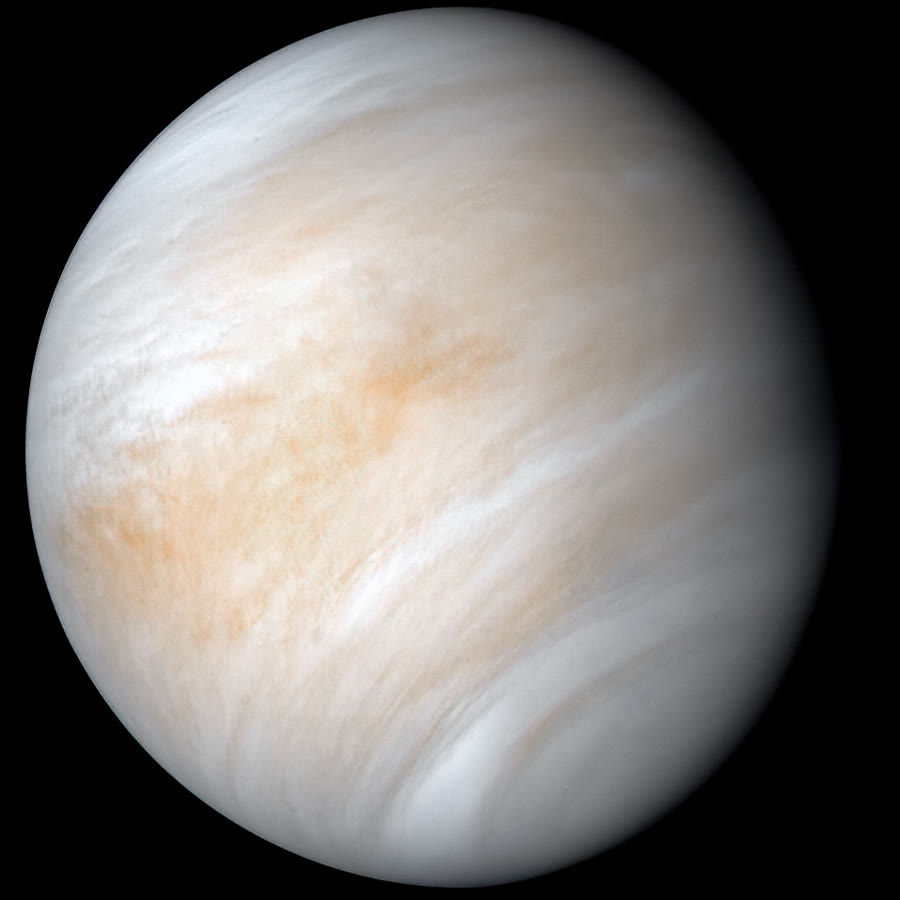
\includegraphics[width=0.38\linewidth]{images/book2/g10-nasa-venus-mariner10.jpg}

{\small 1974 年，探测器 Mariner~10 拍摄的金星，颜色接近人眼所见：
整颗行星被云层完全包裹。图像：NASA/JPL-Caltech
（公有领域）。}
\end{omfigure}

\begin{recall}
太阳是一颗恒星，围绕它运行的有四颗岩质行星：水星、金星、地球和火星，
以及四颗巨行星，它们几乎都沿近圆形轨道运行，
（见物理各册和第 1 册）。任何物体都会以光的形式辐射能量，
温度越高，辐射越多，在行星温度下主要是红外线，
（见物理各册）。温室气体——水蒸气、二氧化碳、甲烷——会吸收
地表所发出的部分红外线，使地表保持较高温度（见化学各册）。
水以冰、液态水和水蒸气的形式存在；压强是单位面积上的力，
以帕斯卡为单位；
（见物理各册）。
\end{recall}

\section{恒星设定的温度}

太阳向各个方向均匀发光。距太阳 $d$ 处，它的
功率 $L$（即\emph{光度}）均匀分布于面积为 $4\pi d^2$ 的球面上。

\begin{proposition}[太阳光的平方反比定律]\label{prop:g10:habitable-planet:inverse-square}
距太阳 $d$ 处，正对太阳的每平方米所接收的功率，即\emph{太阳
辐照度}，为
\[
  S = \frac{L}{4\pi d^2}.
\]
在地球距离 \qty{1}{au} 处，$S_0 = \qty{1361}{W/m^2}$；
若以天文单位计的距离为 $d$，则 $S = S_0/d^2$。
\end{proposition}

\begin{proof}
真空中光不会损失，因此全部功率 $L$ 穿过每个以太阳为中心的球面；
在半径为 $d$ 的球面上，它被分摊到 $4\pi d^2$ 平方米的面积上。
$d$ 加倍时，面积变为四倍，
$S$ 则降为原来的四分之一。
\end{proof}
% ledger: earth:TSI, sun:L, const:au

\begin{omfigure}
\begin{tikzpicture}[font=\small, >={Stealth[length=2mm]}]
  \shade[ball color=yellow!70!orange] (0,0) circle (0.35);
  \node[below=4pt] at (0,-0.35) {太阳};
  \draw[omThm!70, thick] (0,0) -- (3,0.6) (0,0) -- (3,-0.6);
  \draw[omThm!70, thick, dashed] (3,0.6) -- (6,1.2) (3,-0.6) -- (6,-1.2);
  \draw[fill=omDef!25, draw=omDef!80!black] (3,-0.6) rectangle (3.18,0.6);
  \draw[fill=omDef!12, draw=omDef!80!black] (6,-1.2) rectangle (6.18,1.2);
  \draw[omDef!80!black] (6,0) -- (6.18,0) (6.09,-1.2) -- (6.09,1.2);
  \node[anchor=north] at (3.1,-0.7) {$d$};
  \node[anchor=north] at (6.1,-1.3) {$2d$};
  \node[anchor=south east, align=right, font=\footnotesize] at (2.9,0.75) {1 个方格：\\全部光线};
  \node[anchor=west, align=left, font=\footnotesize] at (6.35,0.6) {4 个方格：\\各占四分之一};
  \draw[->, black!60] (0.5,-1.95) -- (6.1,-1.95);
  \node[anchor=north, font=\footnotesize] at (3.3,-2.0) {距太阳的距离};
\end{tikzpicture}

{\small 距离 $d$ 处一个方格所接收的光，分散到距离 $2d$ 处的
四个同样大小的方格中，
辐照度按距离平方的倒数减小。}
\end{omfigure}

行星吸收这些光中未被反射的部分，
并以红外线的形式向太空辐射能量。若吸收的能量多于辐射的能量，
行星就会升温；温度升高后，辐射随之增强；
最终稳定在两者达到平衡的温度上。

\begin{definition}[平衡温度]\label{def:g10:habitable-planet:equilibrium-temperature}
行星的\emph{平衡温度}\index{平衡温度}是指，
一个像完美发射体那样辐射的物体，
其向太空发出的功率恰好等于行星从恒星吸收的功率时的温度。
行星整体反射的入射光所占的比例，即其
\emph{邦德反照率} $A$。
\end{definition}

\begin{proposition}[平衡温度的计算]\label{prop:g10:habitable-planet:teq}
对于将所吸收的热量均匀分布于整个表面的行星，
\[
  T_{\mathrm{eq}} = \left(\frac{S\,(1-A)}{4\sigma}\right)^{1/4},
  \qquad \sigma = \qty{5.67e-8}{W.m^{-2}.K^{-4}}.
\]
在地球距离处且完全不反射时，可得
\qty{278.3}{K}；若以天文单位计的距离为 $d$，反照率为 $A$，则
$T_{\mathrm{eq}} = \qty{278.3}{K} \times (1-A)^{1/4}/\sqrt{d}$。
\end{proposition}

\begin{proof}[部分证明]
行星在面积为 $\pi R^2$ 的圆盘上截获阳光，并吸收
功率 $(1-A)\,S\,\pi R^2$。它从整个表面辐射，面积为 $4\pi R^2$。
温度为 $T$ 的完美发射体，每平方米
辐射 $\sigma T^4$（该定律见物理各册，在本阶段不加证明地承认）。令
$4\pi R^2 \sigma T^4 = (1-A)\,S\,\pi R^2$，即得公式；半径
约去。取 $S = S_0/d^2$，则 $1/d^2$ 的四次方根为 $1/\sqrt d$。
\end{proof}
% ledger: const:sigma, earth:TSI

\begin{example}[地球]\label{ex:g10:habitable-planet:earth}
% ledger: earth:TSI, earth:albedo, earth:Tbb, earth:Tsurf
取 $S_0 = \qty{1361}{W/m^2}$ 和 $A = 0.294$，
$T_{\mathrm{eq}} = 278.3 \times 0.706^{1/4} \approx \qty{255}{K}$，即
\qty{-18}{\degreeCelsius}。（NASA 的数据表给出 \qty{254}{K}。）地球表面的
平均温度为 \qty{288}{K}，
\qty{15}{\degreeCelsius}：大气的温室效应使其升温
约 \qty{33}{K}。若无此效应，海洋将会凝固。
\end{example}

\begin{omfigure}
\begin{tikzpicture}
\begin{axis}[ybar, width=0.86\linewidth, height=5.8cm, ymin=0, ymax=950,
  bar width=10pt, enlarge x limits=0.15, symbolic x coords={Mercury,Venus,Earth,Moon,Mars}, xticklabels={水星,金星,地球,月球,火星},
  xtick=data, ylabel={温度（K）}, ymajorgrids, grid style={gray!22},
  legend style={at={(0.97,0.95)}, anchor=north east, font=\footnotesize, draw=black!30},
  nodes near coords, nodes near coords style={font=\scriptsize, rotate=90, anchor=west, /pgf/number format/fixed, /pgf/number format/precision=0},
  tick label style={font=\small}, label style={font=\small}]
\addplot[fill=omDef!45, draw=omDef!80!black] table[x=name, y=Teq_K] {figdata/out/grade-10-planet_temperatures-planets.dat};
\addlegendentry{平衡温度}
\addplot[fill=omThm!55, draw=omThm!80!black] table[x=name, y=Tmean_K] {figdata/out/grade-10-planet_temperatures-planets.dat};
\addlegendentry{实测平均地表温度}
\end{axis}
\end{tikzpicture}

{\small \omterm{def:g10:habitable-planet:equilibrium-temperature}{平衡温度}由各天体的距离和邦德
反照率算得，与其表面的实测平均温度并列。数据来自 NASA
行星数据表。}
\end{omfigure}

\begin{remark}[读图]\label{rem:g10:habitable-planet:reading}
% ledger: nasa:bond-albedos, planet:Mercury.Tmean, planet:Venus.Tmean, planet:Moon.Tmean, planet:Mars.Tmean, planet:Moon.day, nasa:moon-temps
水星和火星几乎没有大气，或大气极为稀薄，
其实测平均温度接近\omterm{def:g10:habitable-planet:equilibrium-temperature}{平衡温度}。月球的平均温度
低于\omterm{def:g10:habitable-planet:equilibrium-temperature}{平衡温度}：其昼与夜各持续约两周，
其表面温度在约 \qty{95}{K} 与 \qty{390}{K} 之间大幅波动，这一点
简单公式（专为热量均匀分布的行星而作）无法反映。
金星是最突出的例子：邦德反照率为 0.77——其云层反射了
大部分阳光——其\omterm{def:g10:habitable-planet:equilibrium-temperature}{平衡温度}低于
地球的，但其表面温度比地球的\omterm{def:g10:habitable-planet:equilibrium-temperature}{平衡温度}高出 \qty{500}{K} 以上：
这是其浓厚的二氧化碳大气所产生的温室效应。
\end{remark}

\section{留住大气}

气体由不断运动的分子组成，温度越高，分子运动越快。
大气顶层中某个向上运动的分子，其速度超过行星的
逃逸速度——即永久摆脱其引力所需的速度（见物理各册）——
则逸入太空。经过数十亿年，
引力弱的小型行星会失去大气，大行星则将其保留。

\begin{center}
\small
% ledger: planet:Mercury.vesc, planet:Venus.vesc, planet:Earth.vesc, planet:Moon.vesc, planet:Mars.vesc, planet:Mercury.psurf, planet:Venus.psurf, planet:Earth.psurf, planet:Moon.psurf, nasa:mars-atm
\begin{tabular}{lccc}
\hline
天体 & 逃逸速度（\unit{km/s}） & 表面压强（bar） & 大气 \\
\hline
月球 & 2.4 & 0 & 无 \\
水星 & 4.3 & 0 & 无 \\
火星 & 5.0 & 0.006 & 稀薄，二氧化碳 \\
金星 & 10.4 & 92 & 浓厚，二氧化碳 \\
地球 & 11.2 & 1 & 氮气和氧气 \\
\hline
\end{tabular}
\end{center}

\begin{remark}[尺寸并非全部原因]\label{rem:g10:habitable-planet:size}
月球和水星体积小，其中水星又靠近炽热的太阳，几乎已失去全部
气体。火星的逃逸速度为地球的一半，却保留了一层
稀薄的大气。金星与地球的大小和逃逸速度几乎相同，但大气
截然不同：二者的演化历程——其水与二氧化碳的去向——已分道扬镳，
正如在\cref{ch:g12:early-earth}中
就地球所作的说明。
\end{remark}

\section{液态水}

\begin{omfigure}
\begin{tikzpicture}
\begin{axis}[omrecord, width=0.88\linewidth, height=7.2cm, xmin=150, xmax=800,
  ymode=log, ymin=1e-6, ymax=2000, xlabel={温度（K）}, ylabel={压强（bar）},
  xtick={200,300,...,800}, ytick={1e-6,1e-4,1e-2,1,100},
  log basis y=10]
\addplot[omDef!85!black, line width=1.1pt] table[x=T_K, y=p_bar] {figdata/out/grade-10-planet_temperatures-vap.dat};
\addplot[omDef!85!black, line width=1.1pt] table[x=T_K, y=p_bar] {figdata/out/grade-10-planet_temperatures-subl.dat};
\addplot[omDef!85!black, line width=1.1pt] table[x=T_K, y=p_bar] {figdata/out/grade-10-planet_temperatures-melt.dat};
\addplot[only marks, mark=*, mark size=2pt, black] coordinates {(273.16,0.00611657) (647.096,220.64)};
\addplot[only marks, mark=square*, mark size=2.4pt, omThm!85!black] table[x=T_K, y=p_bar] {figdata/out/grade-10-planet_temperatures-points.dat};
\node[font=\small] at (axis cs:205,30) {冰};
\node[font=\small] at (axis cs:420,30) {液态};
\node[font=\small] at (axis cs:600,1e-3) {水蒸气};
\node[font=\footnotesize, anchor=north west] at (axis cs:276,0.0055) {三相点};
\node[font=\footnotesize, anchor=south east] at (axis cs:640,300) {临界点};
\node[font=\footnotesize, anchor=south, omThm!85!black] at (axis cs:737,110) {金星};
\node[font=\footnotesize, anchor=west, omThm!85!black] at (axis cs:296,1.0) {地球};
\node[font=\footnotesize, anchor=north, omThm!85!black] at (axis cs:210,0.0045) {火星};
\end{axis}
\end{tikzpicture}

{\small 水的相图，并标出金星、地球和火星的
平均表面条件（方块）。压强轴为对数刻度，每一刻度为其下方
刻度的一百倍。曲线依据方程计算，方程来自
国际水和水蒸气性质协会；
行星数值来自 NASA。}
\end{omfigure}

\begin{proposition}[水何时为液态]\label{prop:g10:habitable-planet:liquid}
% ledger: iapws:triple-critical, iapws:vapour-pressure, iapws:melt-subl
液态水仅存在于压强高于\emph{三相点}压强的条件下，
该压强为 \qty{611.657}{Pa}（\qty{0.006}{bar}），此时冰、液态水与水蒸气共存于
\qty{273.16}{K}，且温度低于\emph{临界点}，
\qty{647.096}{K}（\qty{220.64}{bar}）处的临界点，超过此点后，液态水与水蒸气
不再能加以区分。在高于三相点的某一给定压强下，水
处于液态，温度介于约 \qty{273}{K} 的熔点与
沸点之间，且沸点随压强降低而下降。
\end{proposition}

\begin{example}[同一图中的三颗行星]\label{ex:g10:habitable-planet:three}
% ledger: nasa:venus-atm, nasa:mars-atm, earth:psurf, earth:Tsurf (boiling point at 636 Pa computed)
地球表面温度为 \qty{288}{K}、压强为 \qty{1}{bar}，位于
液相场之内：该处的水可能随天气变化而呈液态、冰或水蒸气。
金星表面温度为 \qty{737}{K}，远高于临界温度，
因此那里根本不可能存在液态水。火星压强为 \qty{6.36}{mbar}，恰好略高于
三相点：那里的水约在 \qty{0.5}{\degreeCelsius} 沸腾，因此液态水
只能在约半度的温度区间内存在，而平均温度
为 \qty{210}{K}，位于冰相场内。
\end{example}

\begin{omfigure}
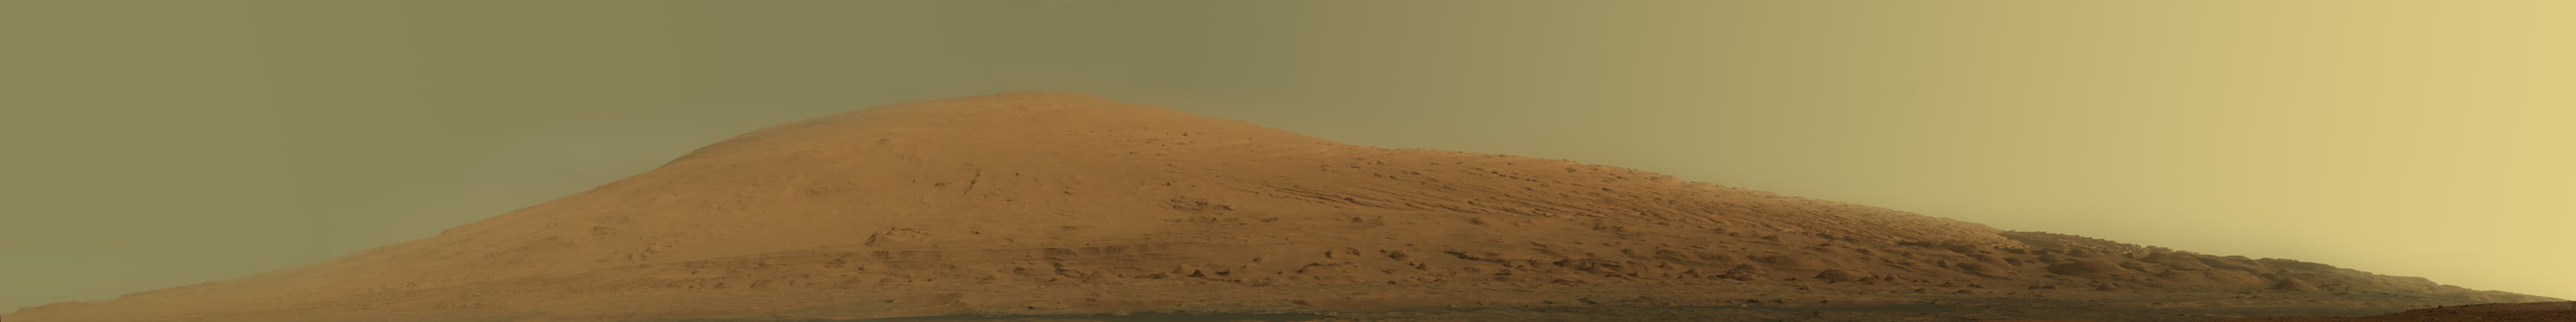
\includegraphics[width=0.96\linewidth]{images/book2/g10-nasa-mars-mount-sharp.jpg}

{\small 火星上盖尔火山口内的夏普山，由好奇号火星车于 2012 年拍摄，
以其照相机记录的颜色显示。其下部
岩层形成于水中，距今数十亿年。图像：NASA/JPL-Caltech/MSSS
（公有领域）。}
\end{omfigure}

\section{宜居带}

\begin{definition}[宜居带]\label{def:g10:habitable-planet:habitable-zone}
恒星的\emph{宜居带}\index{宜居带}是指一段
距离范围，在该范围内，水量充足、大气与地球相似的岩质行星
可在其表面保持液态水。其内缘是行星因受热而失去水分之处；
其外缘是即使很强的温室效应也
无法阻止其
结冰之处。
\end{definition}

\begin{proposition}[太阳的宜居带]\label{prop:g10:habitable-planet:hz-sun}
% ledger: kopparapu:hz-sun, planet:Mercury.dist, planet:Venus.dist, planet:Mars.dist
行星大气的详细模型表明，太阳的\omterm{def:g10:habitable-planet:habitable-zone}{宜居带}
位于 \qty{0.99}{au} 与 \qty{1.70}{au} 之间。地球（\qty{1}{au}）恰好位于
其内缘之内；火星（\qty{1.52}{au}）位于其中；金星
（\qty{0.72}{au}）则远在内缘之内。
\end{proposition}

\begin{proposition}[其他恒星的宜居带]\label{prop:g10:habitable-planet:hz-scaling}
在光度为 $L$ 的恒星周围，行星所接收的辐照度与距太阳
距离为 $d_\odot$ 时相同，此时行星位于
\[
  d = d_\odot \sqrt{L/L_\odot}.
\]
\omterm{def:g10:habitable-planet:habitable-zone}{宜居带}的边界按比例移动，作一级近似时，
（恒星光的颜色也有少许影响。）
\end{proposition}

\begin{proof}
辐照度相等，即 $L/(4\pi d^2) = L_\odot/(4\pi d_\odot^2)$，于是
$d^2 = d_\odot^2\,L/L_\odot$。
\end{proof}

\begin{omfigure}
\begin{tikzpicture}[font=\small]
  % top: the Sun, 0-2 au over 12 cm (6 cm per au)
  \fill[omProp!30] (0.99*6,0) rectangle (1.70*6,0.5);
  \draw[black!70] (0,0.25) -- (12.3,0.25);
  \foreach \x in {0,0.5,...,2} \draw (\x*6,0.15) -- (\x*6,0.35) node[pos=0, below=1pt, font=\footnotesize] {\x};
  \shade[ball color=yellow!70!orange] (0,0.25) circle (0.22);
  \foreach \n/\d in {水星/0.387, 金星/0.723, 地球/1.0, 火星/1.524} {
    \fill[omThm!85!black] (\d*6,0.25) circle (2.2pt);
    \node[anchor=south, font=\footnotesize] at (\d*6,0.55) {\n};
  }
  \node[anchor=west, font=\footnotesize] at (12.4,0.25) {au};
  \node[anchor=north, font=\footnotesize] at (8.07,-0.25) {宜居带，0.99--1.70 au};
  \node[anchor=east, font=\footnotesize] at (-0.3,0.25) {太阳};
  % bottom: Proxima Centauri, 0-0.1 au over 12 cm (120 cm per au)
  \begin{scope}[yshift=-2.2cm]
  \fill[omProp!30] (0.0385*120,0) rectangle (0.0661*120,0.5);
  \draw[black!70] (0,0.25) -- (12.3,0.25);
  \foreach \x/\l in {0/0, 0.025/0.025, 0.05/0.05, 0.075/0.075, 0.1/0.1} \draw (\x*120,0.15) -- (\x*120,0.35) node[pos=0, below=1pt, font=\footnotesize] {\l};
  \shade[ball color=red!70!orange] (0,0.25) circle (0.14);
  \fill[omThm!85!black] (0.0485*120,0.25) circle (2.2pt);
  \node[anchor=south, font=\footnotesize] at (0.0485*120,0.55) {比邻星 b};
  \node[anchor=west, font=\footnotesize] at (12.4,0.25) {au};
  \node[anchor=north, font=\footnotesize] at (6.28,-0.25) {宜居带，0.038--0.066 au};
  \node[anchor=east, align=right, font=\footnotesize] at (-0.3,0.25) {比邻星};
  \end{scope}
\end{tikzpicture}

{\small 上图：太阳的\omterm{def:g10:habitable-planet:habitable-zone}{宜居带}及四颗岩质行星。下图：
暗弱的红色恒星比邻星的\omterm{def:g10:habitable-planet:habitable-zone}{宜居带}，由太阳的\omterm{def:g10:habitable-planet:habitable-zone}{宜居带}
按恒星光度的平方根缩放得到，以及其行星
比邻星~b。注意比例尺已改变：下图整条带
长 \qty{0.1}{au}。}
\end{omfigure}

\section{其他恒星的行星}

\begin{definition}[系外行星]\label{def:g10:habitable-planet:exoplanet}
\emph{系外行星}\index{系外行星}是指绕
太阳以外的恒星运行的行星。
\end{definition}

\omterm{def:g10:habitable-planet:exoplanet}{系外行星}过于暗弱，且离其恒星过近，
难以直接观测，少数巨行星除外。多数\omterm{def:g10:habitable-planet:exoplanet}{系外行星}通过间接方法发现：
或是行星每绕行一周便从其恒星前方经过一次，使恒星略微变暗，
或是行星的引力使恒星朝向或远离我们摆动，从而使恒星光的
颜色来回移动。第二种方法只能给出行星的
\emph{最小}质量，因为轨道倾角
未知。这些方法将在本科三年级分册中学习。

\begin{dated}{2026}
% ledger: nea:count-2026
2026 年 10 月 15 日，NASA Exoplanet Archive 列出已确认的 6\,451
颗\omterm{def:g10:habitable-planet:exoplanet}{系外行星}。
\end{dated}

\begin{example}[比邻星 b]\label{ex:g10:habitable-planet:proxima}
% ledger: nea:proxima-b (flux and habitable zone computed in figdata/grade-10/planet_temperatures.py)
离太阳最近的恒星比邻星，距太阳 \qty{1.30}{\parsec}，是一颗
小红矮星，其光度仅约为太阳的 $0.0015$ 倍。2016 年，
人们在其周围发现一颗行星，每 11.2 天绕行一周，距恒星 \qty{0.0485}{au}，
质量至少为地球的 1.06 倍。在该距离处，它接收到的
辐照度约为地球所接收辐照度的 0.64 倍，并且它位于
其恒星的\omterm{def:g10:habitable-planet:habitable-zone}{宜居带}内。它是否拥有大气或水，目前尚不清楚。
\end{example}

\begin{remark}[宜居不等于有生命]\label{rem:g10:habitable-planet:inhabited}
\omterm{def:g10:habitable-planet:habitable-zone}{宜居带}仅是关于距离和光照的说法。位于\omterm{def:g10:habitable-planet:habitable-zone}{宜居带}内的行星
也可能没有水、没有大气，或大气成分不适宜——火星位于太阳的
\omterm{def:g10:habitable-planet:habitable-zone}{宜居带}内，但今日其表面没有液态水。地球
之所以宜居，是因为多个条件同时满足：距离适当，
质量足够大以保留大气，水量丰富，并有适度的温室
效应，既不过弱，也不过强。
\end{remark}

\section{练习}

\begin{exercise}[$\star$]\label{exo:g10:habitable-planet:1}
给出行星\omterm{def:g10:habitable-planet:equilibrium-temperature}{平衡温度}的定义。为何地球的平均
地表温度高于其\omterm{def:g10:habitable-planet:equilibrium-temperature}{平衡温度}？
\end{exercise}

\begin{exercise}[$\star$]\label{exo:g10:habitable-planet:2}
利用\omterm{def:g10:habitable-planet:equilibrium-temperature}{平衡温度}与实测温度的柱状图，指出
哪一天体表面受大气增温最多，并估算
其升温多少开尔文。
\end{exercise}

\begin{exercise}[$\star$]\label{exo:g10:habitable-planet:3}
火星距太阳 \qty{1.52}{au}。利用平方反比定律，
$S_0 = \qty{1361}{W/m^2}$，计算火星处的太阳辐照度。
\end{exercise}

\begin{exercise}[$\star$]\label{exo:g10:habitable-planet:4}
利用水的相图，给出水在 \qty{1}{bar} 和 \qty{330}{K} 时的状态；
在 \qty{0.001}{bar} 和 \qty{250}{K} 时的状态；在 \qty{100}{bar} 和
\qty{700}{K} 时的状态。
\end{exercise}

\begin{exercise}[$\star$]\label{exo:g10:habitable-planet:5}
什么是\omterm{def:g10:habitable-planet:exoplanet}{系外行星}？请用一句话分别描述探测\omterm{def:g10:habitable-planet:exoplanet}{系外行星}
的两种主要方法。
\end{exercise}

\begin{exercise}[$\star\star$]\label{exo:g10:habitable-planet:6}
计算地球的\omterm{def:g10:habitable-planet:equilibrium-temperature}{平衡温度}，取 $S_0 = \qty{1361}{W/m^2}$，
分别取 $A = 0.294$ 和 $A = 0$，并将两结果换算为摄氏度。
\end{exercise}

\begin{exercise}[$\star\star$]\label{exo:g10:habitable-planet:7}
某恒星的光度是太阳的 4 倍。其\omterm{def:g10:habitable-planet:habitable-zone}{宜居带}位于
哪两个距离之间？若将地球置于距该恒星 \qty{1}{au} 处，
它是否位于\omterm{def:g10:habitable-planet:habitable-zone}{宜居带}内？
\end{exercise}

\begin{exercise}[$\star\star$]\label{exo:g10:habitable-planet:8}
金星距太阳 \qty{0.723}{au}。计算其接收的辐照度，再
用其邦德反照率 0.77 计算\omterm{def:g10:habitable-planet:equilibrium-temperature}{平衡温度}，并与
其表面温度 \qty{737}{K} 比较，解释其差异。
\end{exercise}

\begin{exercise}[$\star\star$]\label{exo:g10:habitable-planet:9}
火星表面平均压强为 \qty{6.36}{mbar}，刚好高于水的
三相点，在此压强下水的沸点约为 \qty{0.5}{\degreeCelsius}。
试解释为何今日火星表面无法长期存在液态水，即使在
夏季午后地面温度达到 \qty{10}{\degreeCelsius} 时亦然。
\end{exercise}

\begin{exercise}[$\star\star$]\label{exo:g10:habitable-planet:10}
月球的逃逸速度为 \qty{2.4}{km/s}，地球的为
\qty{11.2}{km/s}。计算二者之比，并解释为何地球能够保留大气，
而月球却没有。
\end{exercise}

\begin{exercise}[$\star\star$]\label{exo:g10:habitable-planet:11}
假设地球被冰层覆盖，其邦德反照率升至 0.50。
计算其新的\omterm{def:g10:habitable-planet:equilibrium-temperature}{平衡温度}。试解释为何这样的状态一旦
形成，便倾向于持续存在。
\end{exercise}

\begin{exercise}[$\star\star\star$]\label{exo:g10:habitable-planet:12}
证明由本章公式可得 $T_{\mathrm{eq}} = \qty{278.3}{K} \times (1-A)^{1/4}/\sqrt{d}$，
其中 $d$ 以天文单位计。若距离扩大为
原来的四倍，\omterm{def:g10:habitable-planet:equilibrium-temperature}{平衡温度}将变为
原来的多少倍？
\end{exercise}

\begin{exercise}[$\star\star\star$]\label{exo:g10:habitable-planet:13}
反照率为 0.294 的行星，距太阳多远时其\omterm{def:g10:habitable-planet:equilibrium-temperature}{平衡温度}为
\qty{273}{K}？请将结果与\omterm{def:g10:habitable-planet:habitable-zone}{宜居带}内缘比较，
并解释二者为何不同。
\end{exercise}

\begin{exercise}[$\star\star\star$]\label{exo:g10:habitable-planet:14}
某行星表面压强为 \qty{1000}{Pa}，此压强下水的沸点约为
\qty{7}{\degreeCelsius}。水能保持液态的温度范围是
多少？在该行星上，某日气温为
\qty{15}{\degreeCelsius} 时，湖泊会发生什么变化？
\end{exercise}

\begin{exercise}[$\star\star\star$]\label{exo:g10:habitable-planet:15}
一颗行星绕光度为太阳一半的恒星运行，距该恒星
\qty{1.2}{au}。计算该恒星\omterm{def:g10:habitable-planet:habitable-zone}{宜居带}的边界，并判断该行星
是否位于其中。对该结论有多大把握？
\end{exercise}

\section{问题：Proxima~b 能否拥有海洋？}

\begin{problem}[{周末问题——从暗弱红星的光
到其最近行星的温度}]
\label{pb:g10:habitable-planet:1}
% ledger: nea:proxima-b, kopparapu:hz-sun, earth:TSI, earth:albedo, planet:Earth.vesc, nasa:bond-albedos (all results computed in figdata/grade-10/planet_temperatures.py or from the rounded data below)
一名学生阅读行星 Proxima~b 的数据表。该恒星的
光度为 $L = 0.00151\,L_\odot$；行星以 $d = \qty{0.0485}{au}$ 的距离绕行，
公转周期为 11.18 天，质量至少为地球的 1.055 倍。采用
$S_0 = \qty{1361}{W/m^2}$，$\sigma = \qty{5.67e-8}{W.m^{-2}.K^{-4}}$，
太阳的\omterm{def:g10:habitable-planet:habitable-zone}{宜居带} \qtyrange{0.99}{1.70}{au}，以及地球的逃逸速度
\qty{11.2}{km/s}。

\medskip
\noindent\textbf{第一部分——恒星的光。}
\begin{enumerate}
  \item 计算行星处的辐照度与地球处辐照度之比，
        $L/d^2$（其中 $L$ 以太阳光度计，$d$ 以天文单位计）。
  \item 以 \unit{W/m^2} 为单位表示该辐照度。
  \item 将其与金星处的辐照度（\qty{2601}{W/m^2}）和
        火星处的辐照度（\qty{586}{W/m^2}）作比较。
  \item 一个地球年中有多少个该行星的年？
\end{enumerate}

\medskip
\noindent\textbf{第二部分——无大气时的温度。}
\begin{enumerate}[resume]
  \item 计算一颗完全不反光的行星
        （$A = 0$）在该辐照度下的\omterm{def:g10:habitable-planet:equilibrium-temperature}{平衡温度}。
  \item 计算与金星一样明亮的行星（$A = 0.77$）的\omterm{def:g10:habitable-planet:equilibrium-temperature}{平衡温度}。
  \item 两个温度中，哪一个高于水的凝固点？
        这两个结果说明了云与
        冰的作用是什么？
\end{enumerate}

\medskip
\noindent\textbf{第三部分——\omterm{def:g10:habitable-planet:habitable-zone}{宜居带}。}
\begin{enumerate}[resume]
  \item 计算 $\sqrt{L/L_\odot}$。
  \item 计算该恒星\omterm{def:g10:habitable-planet:habitable-zone}{宜居带}的内边界。
  \item 计算其外边界。
  \item Proxima~b 是否位于\omterm{def:g10:habitable-planet:habitable-zone}{宜居带}之内？
  \item 行星距太阳多远时会接收到与
        Proxima~b 相同的辐照度？该位置在太阳
        \omterm{def:g10:habitable-planet:habitable-zone}{宜居带}中的何处？
\end{enumerate}

\medskip
\noindent\textbf{第四部分——大气与水？}
\begin{enumerate}[resume]
  \item 若该行星的平均密度与地球相同，则其半径为地球的
        $1.055^{1/3}$ 倍。计算该因子。
  \item 逃逸速度与 $\sqrt{M/R}$ 成正比。估算
        该行星的逃逸速度。它能否保留大气？
  \item 为什么该行星的质量只能给出下限？
  \item 在相图上，能使液态水存在的最低表面压强
        为多少？
  \item 取地球的反照率，计算 Proxima~b 的
        \omterm{def:g10:habitable-planet:equilibrium-temperature}{平衡温度}（反照率取 0.294）。
  \item 要使其表面达到地球的平均温度，其温室效应
        须将其升高多少开尔文，
        地球平均温度为 \qty{288}{K}？
\end{enumerate}
\end{problem}
